%% Version 4.3.1, 19 May 2014
%
%%%%%%%%%%%%%%%%%%%%%%%%%%%%%%%%%%%%%%%%%%%%%%%%%%%%%%%%%%%%%%%%%%%%%%
% Template.tex --  LaTeX-based template for submissions to the 
% American Meteorological Society
%
% Template developed by Amy Hendrickson, 2013, TeXnology Inc., 
% amyh@texnology.com, http://www.texnology.com
% following earlier work by Brian Papa, American Meteorological Society
%
% Email questions to latex@ametsoc.org.
%
%%%%%%%%%%%%%%%%%%%%%%%%%%%%%%%%%%%%%%%%%%%%%%%%%%%%%%%%%%%%%%%%%%%%%
% PREAMBLE
%%%%%%%%%%%%%%%%%%%%%%%%%%%%%%%%%%%%%%%%%%%%%%%%%%%%%%%%%%%%%%%%%%%%%

%% Start with one of the following:
% DOUBLE-SPACED VERSION FOR SUBMISSION TO THE AMS
%\documentclass{ametsoc}

% TWO-COLUMN JOURNAL PAGE LAYOUT---FOR AUTHOR USE ONLY
 \documentclass[final]{ametsoc}
 \usepackage[colorinlistoftodos]{todonotes}
 \usepackage{booktabs}
 %\usepackage{graphicx}
%%%%%%%%%%%%%%%%%%%%%%%%%%%%%%%%
%%% To be entered only if twocol option is used

\journal{bams}

%  Please choose a journal abbreviation to use above from the following list:
% 
%   jamc     (Journal of Applied Meteorology and Climatology)
%   jtech     (Journal of Atmospheric and Oceanic Technology)
%   jhm      (Journal of Hydrometeorology)
%   jpo     (Journal of Physical Oceanography)
%   jcli      (Journal of Climate)
%   mwr      (Monthly Weather Review)
%   wcas      (Weather, Climate, and Society)
%   waf       (Weather and Forecasting)
%   bams (Bulletin of the American Meteorological Society)
%   ei    (Earth Interactions)

%%%%%%%%%%%%%%%%%%%%%%%%%%%%%%%%
%Citations should be of the form ``author year''  not ``author, year''
\bibpunct{(}{)}{;}{a}{}{,}

%%%%%%%%%%%%%%%%%%%%%%%%%%%%%%%%

%%% To be entered by author:

%% May use \\ to break lines in title:

\title{A containerized mesoscale model and analysis toolkit to accelerate classroom learning,
collaborative research, and uncertainty quantification}

%%% Enter authors' names, as you see in this example:
%%% Use \correspondingauthor{} and \thanks{Current Affiliation:...}
%%% immediately following the appropriate author.
%%%
%%% Note that the \correspondingauthor{} command is NECESSARY.
%%% The \thanks{} commands are OPTIONAL.

%    \authors{Author One\correspondingauthor{Author One, 
%     American Meteorological Society, 
%     45 Beacon St., Boston, MA 02108.}
% and Author Two\thanks{Current affiliation: American Meteorological Society, 
%     45 Beacon St., Boston, MA 02108.}}

\authors{Joshua P. Hacker\correspondingauthor{Joshua P. Hacker, Research Applications Laboratory, NCAR, P.O. Box 3000, Boulder, CO 80307.} John Exby, David Gill}


%% Follow this form:
    % \affiliation{American Meteorological Society, 
    % Boston, Massachusetts.}

\affiliation{Research Applications Laboratory, National Center for Atmospheric Research, Boulder, CO.}

%% Follow this form:
    %\email{latex@ametsoc.org}

\email{hacker@ucar.edu}

%% If appropriate, add additional authors, different affiliations:
    %\extraauthor{Extra Author}
    %\extraaffil{Affiliation, City, State/Province, Country}

\extraauthor{Ivo Jimenez, Carlos Maltzahn}
\extraaffil{Computer Science Department, University of California Santa Cruz}

%% May repeat for a additional a uthors/affiliations:

\extraauthor{Timothy See, Gretchen Mullendore}
\extraaffil{Department of Meteorology, University of North Dakota}


%%%%%%%%%%%%%%%%%%%%%%%%%%%%%%%%%%%%%%%%%%%%%%%%%%%%%%%%%%%%%%%%%%%%%
% ABSTRACT
%
% Enter your Abstract here

\abstract{Numerical weather prediction (NWP) experiments can be complex and time consuming; results depend on computational environments and numerous input parameters. Delays in learning and obtaining research results are inevitable. Students face disproportionate effort in the classroom or beginning graduate-level NWP research. Published NWP research is generally not reproducible, introducing uncertainty in the results, and slowing efforts that build on past results. This work exploits the rapid emergence of software container technology to produce a transformative research and education environment. The Weather Research and Forecasting (WRF) model anchors a set of linked Linux-based containers, which include software to initialize and run the model, analyze results, and serve output to collaborators. The containers are demonstrated with a WRF simulation of Hurricane Sandy. The demonstration illustrates the following: (1) how the often-difficult exercise in compiling the WRF and its many dependencies is eliminated ; (2) how sharing containers provides identical environments for conducting research; (3) that numerically reproducible results are easily obtainable; and (4) how uncertainty in the results can be isolated from uncertainty arising from computing system differences. Numerical experiments to simultaneously measure numerical reproducibility and sensitivity to compiler optimization provide guidance for interpreting NWP research. Reproducibility is independent from operating system and hardware. Results here show numerically identical output on all computing platforms tested. Performance reproducibility is also demonstrated. The result is an infrastructure to accelerate classroom learning, graduate research, and collaborative science.}

\begin{document}

%% Necessary!
\maketitle


%%%%%%%%%%%%%%%%%%%%%%%%%%%%%%%%%%%%%%%%%%%%%%%%%%%%%%%%%%%%%%%%%%%%%
% MAIN BODY OF PAPER
%%%%%%%%%%%%%%%%%%%%%%%%%%%%%%%%%%%%%%%%%%%%%%%%%%%%%%%%%%%%%%%%%%%%%
%

%% In all cases, if there is only one entry of this type within
%% the higher level heading, use the star form: 
%%
\section{Introduction}

Numerical models are a cornerstone of weather prediction today, and also support a broad range of weather research. Studies quantifying the ability of numerical models to predict atmospheric state, and simulate atmospheric phenomena, form two key lines of inquiry. By establishing model fidelity to the atmosphere, those studies also provide a basis for broader scientific inquiry with models. The use of numerical models in atmospheric research has become ubiquitous over the past few decades. Areas of research include physical process identification and analysis, atmospheric predictability, and predictions of future climates, among others.  

Extensive use of numerical models in research demands educating students for diligent application of these large and complex codes. Beyond basic theory and practice in numerical methods, correctly executing simulations is difficult for inexperienced researchers. The opportunities to make mistakes are vast.  While mistakes can provide positive learning experiences, they can also lead to misleading results and consequently incorrect interpretation.  

This contribution describes implementation of software containers for numerical weather prediction (NWP) research and education. Container technology has profound implications for education and research in numerical weather prediction. Containers not only enable reproducibility, they greatly lower barriers for accessing cutting edge NWP codes. 

The Weather Research and Forecasting (WRF) model \citep{Skamarock:08} is a state-of-the-science numerical weather prediction (NWP) model for operations and research, with users numbering in the tens of thousands. It was engineered to be portable and easy to install on a limited yet common set of platforms, the code is complex (over 1.5 million lines) and has many dependencies on external software packages (e.g.\@ for I/O, parallel communications, and data compression) that are not trivial to satisfy; compilation and execution can be an intensive effort for beginning users who lack support from experienced system administrators. The WRF help-desk requests are dominated by new users with difficulty compiling the model. A new version has been released twice annually for the last 15 years, and users who want to update and rebuild may face repeated challenges with each new set of code. 

Running the model can also be difficult for new users.  Individual steps to generate computational grids, import initialization data, produce initial and boundary conditions, and run the model can be daunting.  Those steps can be scripted into a workflow that can range from simple to complex, depending on the application.  Scripted workflows have been developed by countless individuals and groups over the last decade; the proverbial ``wheel" has been reinvented countless times, especially when considering the number of individuals who have written analysis tools to compute the same diagnostics on output.

Implementation of experiential learning with numerical weather prediction is especially challenging for users in the classroom.  Some universities are able to provide hands-on exercises due to a combination of sufficient lab resources and, most importantly, staff (faculty and support) with a sufficient knowledge base in modeling and information technology.  But even those universities with sufficient knowledge struggle with continual updates to compilers, operating systems, and model code.  

Results from software that implements floating point operations is generally not  numerically reproducible. Examples of the impacts on numerical weather models can be found in \citet{Thomas02} and \citet{Baker:2015}. A consequence is that NWP research is not reproducible, despite the number of peer-reviewed articles that present results from NWP experiments. 

The same numerical uncertainty can lead to misleading results. The chaotic nature of the models means that small perturbations, perhaps arising from truncation errors, can organize and grow into features that are tempting to interpret as an important experimental response to a change in input or model formulation. Many times the differences appearing meaningful cannot be reproduced, or simply cannot be distinguished from luck.

Finally, collaboration amongst researchers working on different computing platforms can be cumbersome. It often relies on careful, manual, code management to make sure collaborators are working with the same code. Configuration of a complex model must also be done carefully, and still the opportunity to make mistakes is always present. Often, large tar files need to be shared via exposed ftp servers.  

Software containers, which are becoming an essential part of modern software development and deployment, offer a path for mitigating or eliminating many of the problems in NWP research and education that are described above.  In the remaining text, we describe how and show some examples. First, software containers are reviewed. Then in section \ref{sec:WRFcontainers} a set of containers for initializing, running, and analyzing results from the WRF model are presented.  Section \ref{sec:Sandy} presents an example implementation for a simulation of Hurricane Sandy. Numerical and performance reproducibility are demonstrated in section \ref{sec:performance}, leading to a clear way to perform uncertainty quantification in section \ref{sec:uncertainty}. Section \ref{sec:discussion} concludes with some discussion of the implications for container technology in numerical simulation and prediction. Finally in section \ref{sec:resources}, links to on-line content and open repositories are provided.

\section{Software containers}\label{sec:containers}

Linux containers  have been used in cloud services for over 10 years to provide stability, scalability and a more secure, isolated run-time environment than is often possible on commonly used computing platforms. Today's container engines have defined a homogeneous and emerging standard, which can execute pre-built codes within every modern operating system (OS) including Windows, Mac OS X, and Linux.  Containerized applications provide a well-documented command set that users can implement quickly without regard to a destination OS.  Software deployment methods are simple, and reduce the amount of introduction needed to bring new users or developers into a collaborative group desiring to implement or adopt scientific model improvements or new sets of computer codes.  

Industry experts believe containers will continue to be prevalent, with accelerating adoption due to best-fit scaling on desktops/laptops. Commercial and research cloud platforms are providing greater off-the-shelf server resources as hardware prices either fall, or computing power per dollar spent rises. Container technology is a natural fit to commercial cloud services; a user can immediately deploy software without any knowledge of the underlying hardware or OS. Once software tools are in containers, users have easy access to vast resources of cloud computing, which can be exploited when conditions demand.

The choice of implementing scientific software inside containers provides numerous relevant technical advancements, the most important of which is consistent software run-time environments. We choose Docker (www.docker.com) as the container engine for this work, but others are available.
%Linux containers have a longer history more widely known, and have been used in cloud services for over 10 years to provide stability, scalability and a more secured isolated runtime environment.  Combining these features along with the cross-platform adoption that Docker has raised across the industry, being able to deliver complex pre-compiled scientific models and data sets which can execute anywhere - from ``Windows to Macs to linux to cloud Virtual Machines'' enables users to focus on running scientific analysis with reproducibility, reduced friction of start up times, and software configurations that are now effectively integrated into the workflow and are infinitely portable. Docker containers are based on Linux containers. 
Docker containers are user-friendly, already widely adopted across the industry, and allow users to execute complex pre-compiled scientific codes and access data sets anywhere. The combination of all these features enables users to focus on running numerically reproducible scientific analysis, and to reduce start up times. Within containers, software configurations can be easily integrated into arbitrary workflows that assemble trivially portable modules. Container engines such as Docker ensure that a clean, secured application scan be downloaded by each member of a collaborative team. The containers may use differing data sets assigned at launch, and be built on demand. The resulting output can be stored with metadata using local storage, proven distributed storage technologies, or cloud storage such as Amazon Web Services (aws.amazon.com) S3, Glacier and similar resources.   

The open-source community and the rapid adoption of Docker (and similar) container technologies has boomed since 2012, with entire companies such as Uber, Netflix, Goldman Sachs, and others leveraging containers across hybrid (on premise and cloud) platforms to provide continuous services at remarkable and dynamic scales that can be based on users (or events) worldwide.  Frameworks for managing complex and multiple instances of containers are evolving to provide streamlined tools for users and developers that allow flexibility, verification, reporting and coordination across an enterprise level of processing.    


% * <hacker@ucar.edu> 2016-05-19T15:59:09.174Z:
%
% > similar data container technology methods
%
% I don't understand what this means.
%
% ^ <hacker@ucar.edu> 2016-05-19T15:59:38.133Z.

Prior to June 2016, the released and stable Docker engine stack for Windows and Mac OS X required a thin virtual machine (VM) layer managed by VirtualBox (www.virtualbox.org), in order to pass container commands to a Linux VM environment.
The VM layer added a slight performance loss (approx. 5\% in run time), and it also created extra docker-machine configuration and management steps often not familiar to general users. As of June 2016, new (v.1.10+ beta and beyond) versions of Docker (engine) for Windows and Mac OS X have bypassed the requirement of a Linux VM, completely discarding Virtualbox, and all local Docker-machine management and VM configuration steps. This allows Docker containers to run natively on Windows and OS X platforms, eliminating the slight performance penalty of VMs and delivering container commands to native Windows and OS X kernels. Docker continues to build upon this new beta software for the purposes of incorporating the same native features across Linux, Windows, and OS X.

\section{A set of containers for numerical weather prediction}\label{sec:WRFcontainers}

The Docker containers described above have been implemented so that a user can easily complete a WRF run. The initial set of containers is summarized in the schematic Fig.\@ \ref{Fig:Containers}. So far the WRF-Docker infrastructure includes the WRF and WRF Pre-processing System (WPS) each in containers. A container with the NCAR Command Language (NCL; www.ncl.ucar.edu) based plotting scripts is also implemented. The remaining containers for acquiring input data, archiving output, and sharing output, are in progress in collaboration with several universities under the NSF-funded Big Weather Web project (bigweatherweb.org).   

\begin{figure}
\begin{center}
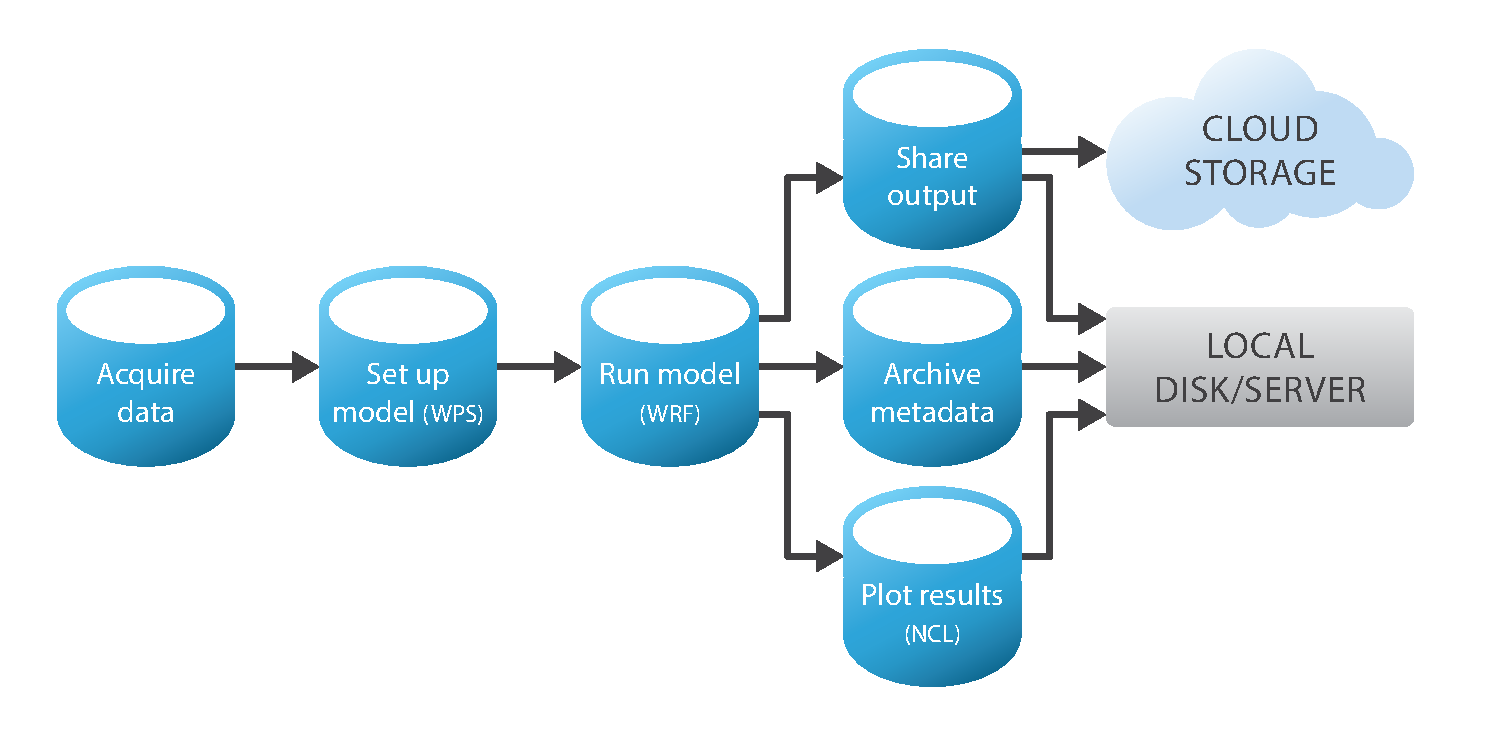
\includegraphics[clip,viewport=20 0 700 360,scale=0.65]{figures/Fig01.pdf}
\caption{\label{Fig:Containers} Schematic illustrating the WRF deployment in a Docker container. It includes set up (pre-processing via the WRF Pre-processing System WPS) and post-processing graphics with NCAR Command Language (NCL) scripting.}
\end{center}
\end{figure}

A user can choose which WRF container to deploy, from one that has a pre-built binary (wrf.exe) and one that has the full source code, gnu compiler, and dependencies. The latter is necessary for users who want to make code modifications, and it is simple to enter a container and make changes. Both containers include the model initialization step (real.exe or its code). They also allow easy run-time configuration by providing external access to the WPS and WRF namelists. The WPS container includes utilities to create domains, populate files with geographical and land-surface data, and interpolate input meteorological data to the WRF computational grid. In the interest of making each container as small as possible, work is in progress to make the containers more granular. For example, the three utilities within the WPS will be split into containers each component, and the model initialization will be separated from the WRF run. 

The schematic in Fig.\@ \ref{Fig:Containers} is arranged as an example workflow, which is easily run from the command line or scripted. The intent is for users to be able to deploy any number of the containers, and substitute his own at any step in the workflow. For example we can imagine that a user may want to introduce a different and more sophisticated post-processing approach that allows analysis supporting a physical  process study. That new container would be deployed in exactly the same way as long as it only needs access to the WRF output files, and the results would be archived or shared in the same way. 

Within the spirit of a community and open-source effort, our vision is that users can contribute useful containers so that others can reproduce results or address other scientific questions with similar tools. The question a researcher often faces, of developing his own code or trying to adapt and port code developed by others, will go away in many cases because no porting effort is required. 

Source codes for the model and ancillary systems, the containers, and data sets (e.g. the geography data needed to design WRF domains) are managed in version-controlled source repositories, which allow continuous integration and unit testing through the chain of source commits to Docker-build image generation.  We choose GitHub (GitHub; www.github.com), but could have equally chosen another repository host such as Bitbucket (www.bitbucket.org) or GitLab (gitlab.com). The GitHub repositories are for developers, or researchers who want to interact with the code to address specific scientific questions. When a project on GitHub is executed to produce a Docker image, the resulting image is pushed to DockerHub, which manages Git repositories for Docker images. Again, we could have equally chosen an Amazon or Google registry service for hosting the Docker images. A user who is not interested in developing (e.g.\@ changing the WRF code or analysis tools) can simply pull images and run them with any necessary run-time input files (namelists, gridded data, etc). Keeping all known fixes and build environments updated, patched and tested through a quality assurance process via a core development team, including code commits to a GitHub repository and pulls from a DockerHub image repository, guarantees software integrity in the launch environment for model results to be replicated, or queried, for future studies.

By the time this paper is in print we expect access to the DockerHub images, and GitHub source and data repositories, to be open.  The version control system ensures bit-perfect results can be obtained across native OS platforms, also that users are accessing an identical code base as required. All collaborators in a group can be sure they are using identical codes and even binaries, providing unambiguous interpretation of quantitative analysis of output from the model or set of analysis tools.

Collaboration on research, which may or may not require code changes, is easily enabled via Github, DockerHub, and the reproducibility properties inherent to working in containers. Collaborators can maintain a repository with version control on the code and container. Mistakes from accidentally using different code bases can be minimized or eliminated by ensuring codes are regularly pushed to, and pulled from, the repository. As we show below in section~\ref{sec:performance}, including the containers in the overall repository strategy ensures that collaborators can perfectly reproduce each other's simulations.

\section{An example container simulation: Hurricane Sandy}\label{sec:Sandy}

Experimentation in the following sections is based on a computationally inexpensive WRF simulation of Hurricane Sandy.  The simulation is on a single computational $50\times50$ horizontal domain with $\Delta X=40$~km and 60 vertical levels. Initial and boundary conditions are interpolated from NCEP's Global Forecast System (GFS). Twelve-hour simulations are initialized at 1200 UTC 27 Oct 2012.  Details of the complete sub-grid and forcing schemes (known as ``physics'') are unimportant here, but they do represent a reasonable set with components widely found in the literature. This computationally inexpensive simulation serves to illustrate the capability, and any of the parameters are trivial to change. A plot of total precipitation accumulated over the 12-h simulation, shown in Fig.~\ref{Fig:Sandy}, is also useful to see the computational domain. The very same container demonstrated here can be trivially used to execute other WRF simulations simply by changing the input data and namelists.

\begin{figure}
\begin{center}
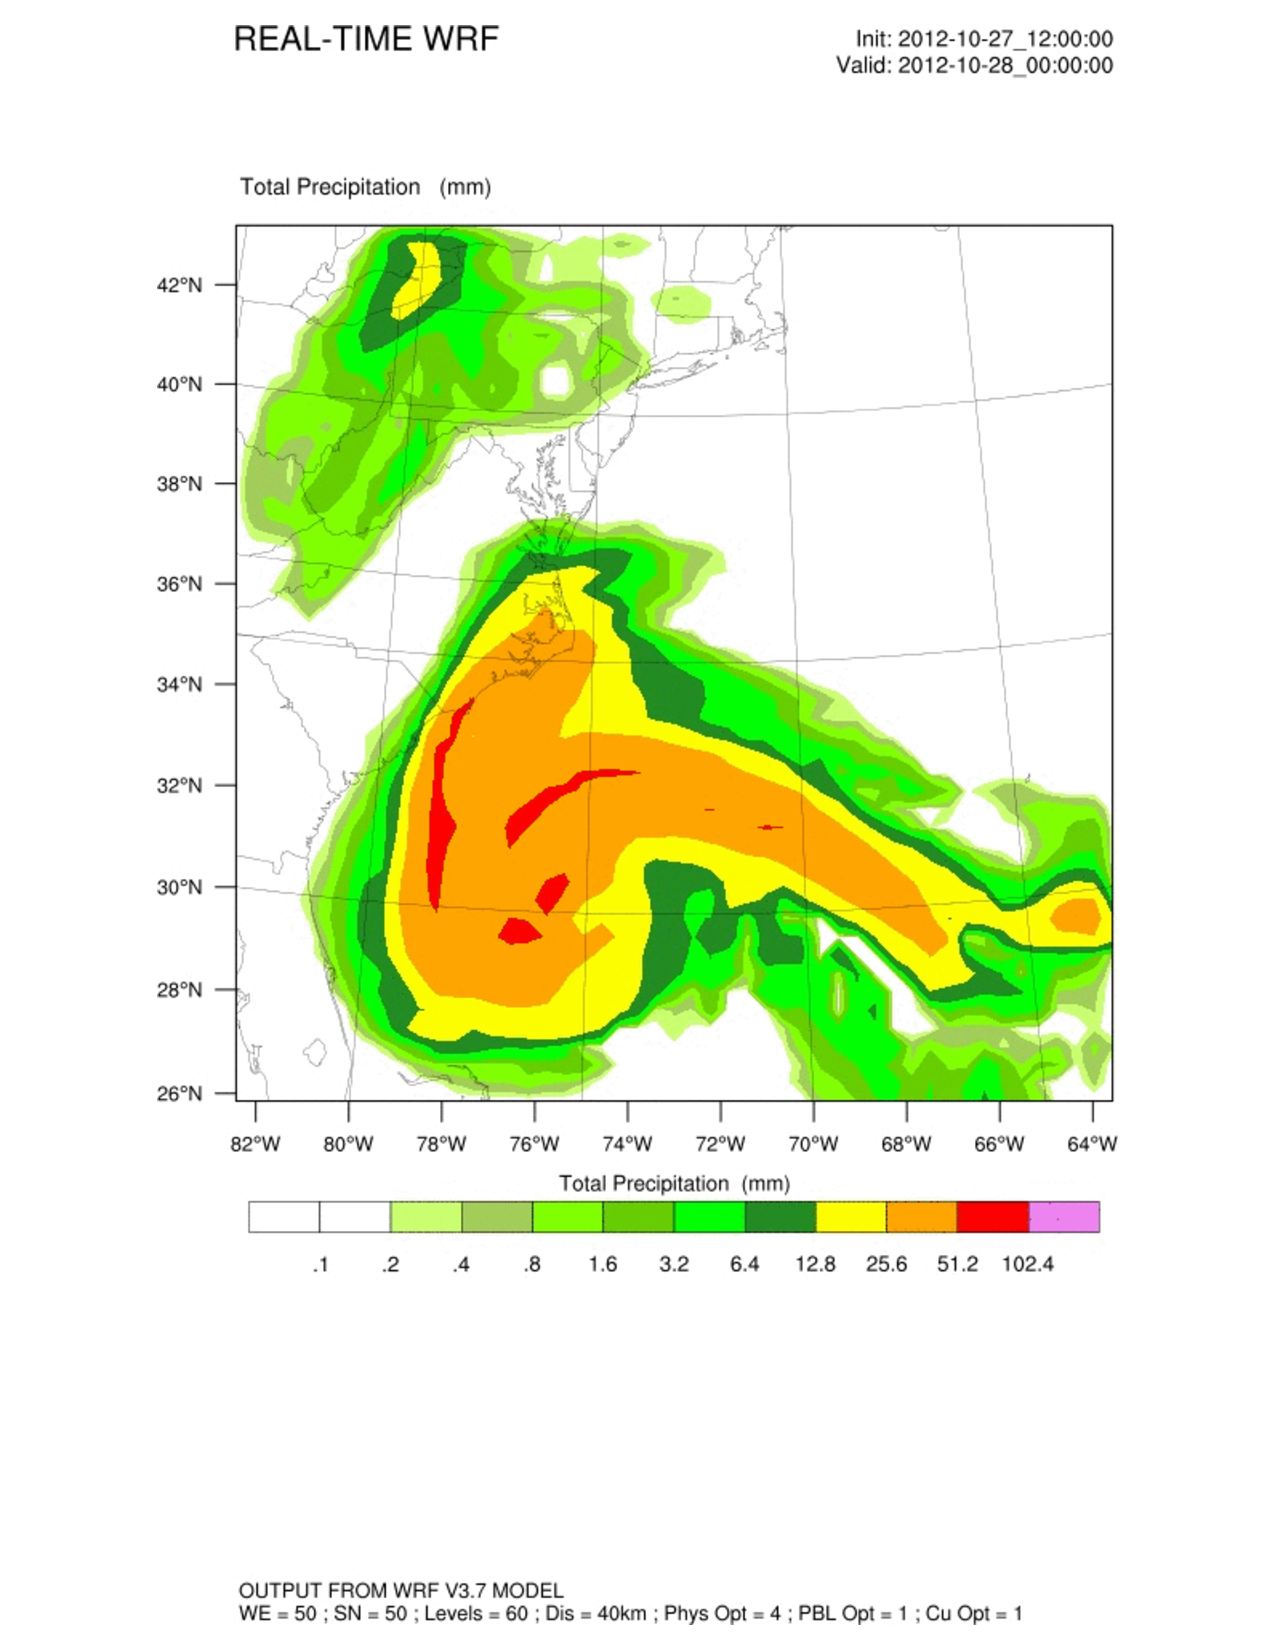
\includegraphics[clip,viewport=60 180 600 690,scale=.3]{figures/Fig02.pdf}
\caption{\label{Fig:Sandy} Simulated 12-h total precipitation from the demonstration Hurricane Sandy simulation, valid 0000 UTC 28 Oct 2012.}
\end{center}
\end{figure}


\section{Numerical and performance reproducibility} \label{sec:performance}

One of the primary reasons that NWP research has historically been numerically non-reproducible is that different computer architectures and environments perform mathematical operations differently.  Differences can be greater when parallel operations are included.  First, different chips have different binary truncation, leading to different effects of round-off error. Second, compilers sometimes reorder operations in attempts to speed computation; the reordering depends on the compiler brand, version, and level of optimization.  Third, unless carefully implemented, parallel operations may not be performed in the same order as intended.  Often this is not a requirement, but truncation guarantees that some computations are not reproducible when the order of a parallel computation is not enforced. For example, the result of an average depends on the precision in the sum and division, and in which order they are performed.  \citet{Thomas02} provides an example of the effect of compiler optimization and parallel topology on NWP, and \citet{Baker:2015} shows how lack of numerical expected numerical uncertainty can indicate deficient code quality. Experiments described here test uncertainty introduced by different hardware and operating systems, parallel topology, and compiler options.  

The Sandy container simulation has been tested on dozens of different computers with a variety of hardware and operating systems.  Table~\ref{Ta:Platforms} shows a small representative sample, including commonly Mac and Linux platforms. It also includes resources available on Amazon's EC2 and Packet's (www.packet.net) Tiny Atom cloud computing infrastructure. Successful deployment and testing is far more extensive than shown in Table \ref{Ta:Platforms}. 

In each case, the same container is deployed and executed. Hourly WRF output files are saved on a user's file system by externally linking to the WRF output directory within the container's file system. An arbitrary platform is chosen as  a reference, which serves as comparison for all of the other test deployments. A deployment in OS X 10.10.5 (Yosemite), with an Intel Xeon E5 on a Mac Pro, serves as the reference here. Free gnu compilers, namely gfortran and gcc, are part of the container for building the WRF executable. Because the compiler and compiler flags are the same, the binary WRF executable is identical regardless of what computer compiles it.  But it is not necessarily obvious that the same binary will produce the same output on different hardware.  


%We have yet to produce in 

\begin{table}\caption{\label{Ta:Platforms} Representative sample of container test platforms for the Hurricane Sandy simulations. An asterisk denotes a deployment on an Amazon EC2 resource; the others are on a laptop or desktop/server. A double asterisk denotes a deployment on a Packet Tiny Atom resource.}
\begin{tabular}{lll}
\hline\hline
OS & Chip/CPU & Cores \\
\hline
OS X 10.10.5 & Intel Xeon E5 & 6 \\
OS X 10.9.5 & Intel Core i7 & 2 \\
Ubuntu 14.04 & AMD Opteron 6320 & 16 \\
Ubuntu 14.04 & Intel Xeon E5 & 16 \\
RHEL & Intel Xeon X5550 & 8 \\
*Ubuntu 14.04 & Intel Xeon E5-2666 v3 & 32 \\
**Ubuntu 14.04 & Intel Atom C2550 & 4 \\
\hline\hline
\end{tabular}
\end{table}

Numerical differences between the reference deployment and any other deployment are simple to compute with any variety of binary difference utility, such as the Unix cmp or checksum, or the netCDF differencing operator ncdiff. In all testing so far and regardless of computing system, all of the WRF output files from the same configuration are bit-wise identical for a particular simulation output hour. 

A container that builds the WRF internally, via the gnu compilers that are inside the container, can equally be deployed on any platform that supports containers.  Experiments have shown that those results are also identical to the output from pre-built binaries deployed as above.  

Container deployment on individual servers, regardless of the number of CPUs or computational cores, also yield identical results. Both the container technology, and also that the WRF code is sufficiently mature to make the same calculations on any parallel topology, are responsible for that result.  Numerical reproducibility across different parallel topologies is non-trivial for such a complex code \citep[e.g.\@][]{Thomas02}, and the WRF developers deserve credit. We have not tested all possible configurations of the WRF, which number in the tens of thousands, so cannot guarantee that all configurations are robust to differences in parallel topologies.

Results from the cross-platform testing here show that numerical reproducibility is easy to achieve with containers, within some easily controlled limitations that are discussed next.  By wrapping all dependencies in a container, researchers working on disparate local hardware, OS, and compiler resources can obtain numerically identical results.   

Containers are an attractive upgrade from virtual machines because the computational overhead is significantly less. In an extensive analysis, \citet{Felter:2014} found that configured properly, Docker containers surpassed Kernel-based Virtual Machines (KVM) in every performance test. Computational and memory performance overhead is very small, and any performance penalty is on I/O and interactions with the operating system. Although OS interactions are negligible for NWP models, I/O can be a limitation. Fortunately the overhead is dependent on the number of I/O operations, not the I/O size.  In many relevant problems the WRF does not output many files, but it can output large files for large computational domains.

In tests on the Sandy simulation we also find minimal performance impact from running within the Docker container. Using identical binary executables inside and outside the container four times on a Linux server, the showed a 3.6\% overhead on wall-clock time when running in the container. The overhead will be greater for operating systems requiring a VM layer (e.g.\@ Windows). 

This Sandy simulation requires relatively few floating-point operations, compared to model executions in typical research and operational NWP today. On a Macbook Air as described in the second line of Table \ref{Ta:Platforms}, the sequence of pulling the container from the repository, running the WRF, and making plots takes approximately 4 minutes. The example demonstrates the potential for classroom utility.

Performance reproducibility can be contrasted with the numerical reproducibility examined above. Performance reproducibility deals with the issue of obtaining the same performance (run time, throughput, latency, etc.) across executions. Reproducing performance is important for gaining accurate evaluations of that performance. For example, when performance improvements to the WRF code base are implemented, evaluating improvements is difficult because it is difficult to account for the changes in hardware over time. In ~\cite{Jimenez1605:Characterizing}, the authors introduce a framework to control the cross-platform variability arising from changes in CPU architectures and generations. This technique leverages Linux's cgroups technology (an underlying component of Docker), which allows a user to specify the CPU bandwidth associated with a container. For example, one can constrain a WRF container to have 50\% the capacity of a CPU core (instead of 100\%, the default behavior). With this feature, one can find the amount of CPU capacity that emulates the behavior of a slower/older machine. Table ~\ref{Ta:perf_repro} shows the results of applying this technique to reproduce the performance of the Hurricane Sandy simulation on multiple platforms.

In Table ~\ref{Ta:perf_repro}, machine issdm-6 is the base system where a reference was executed. When this same simulation is re-executed in other (newer) machines, we observe an inherent speed-up in run time from the improvements in newer CPU technology. For example, machine dwill improves the run time of the original execution by approximately 2.8 times. Using the CPU calibration techniques introduced in ~\cite{Jimenez1605:Characterizing}, which leverages the OS-level virtualization in containers, we carefully constrain the CPU of the machines and re-execute the simulation. The CPU limits column denotes whether the execution was constrained in order to emulate the behavior of the base machine. For the case of dwill, the limitations on CPU bandwidth bring the run time down to the same of the original execution time, closely resembling the original performance.

\begin{table}\caption{\label{Ta:perf_repro} Run time of container executions for the Hurricane Sandy simulations on multiple machines. The normalized run time is the ratio between the reference system \texttt{issdm-6} and the platform identified in the particular row.}
../../experiments/performance_reproducility/perf_reproducibility_table.tex
\end{table}

Performance reproducibility also enables planning for computing needs. This is becoming more important as cloud computing becomes more prevalent. Commercial cloud vendors such as Amazon Web Services, Packet, Google Kubernetes (kubernetes.io), and Microsoft Azure (azure.microsoft.com) generally support container deployment. A researcher or company writing a proposal that may include a need for cloud computing resources can get accurate estimates of performance, and expect it to hold on the variety of hardware offered by vendors.

This section presented a subset of results from runs on many different machines.  Although parallel WRF runs have been part of the testing, they are limited so far to single shared-memory nodes. Distributed Message Passing Interface (MPI) for WRF within Docker containers is under investigation. Progress depends on the MPI-based WRF application having awareness of other linked WRF executables in other containers that may be part of a collective container group. Currently MPI does not have that capability, although Docker containers can be made aware of parallel containers within a collective. 

\section{Uncertainty quantification}\label{sec:uncertainty}

Numerical and performance reproducibility is possible by deploying NWP in containers, enabling a precise quantification of uncertainty from other factors. The reproducibility means that by leveraging available computer power wherever it is available, hundreds or thousands of simulations can be produced with perturbations introduced in initial conditions or model configurations. Such an ensemble would reflect only the perturbations given to it, and not be contaminated by random or systematic errors introduced from traditional computing platforms or changing compiler options.  Leaving ensemble investigations for future work, here we examine the effects of compiler optimization. The effects we report here are certain to be reproducible across many computing platforms. 

A simple pair of simulations illustrate the effects of compiler optimization on numerical predictions. The basic FORTRAN optimization flag for the gnu compiler was successively set to levels from 0 to 3, which is the typical range for compilers.  Setting -O0 forces the compiler to avoid optimizing calculations and memory access, and -O3 allows the compiler a number of relatively aggressive optimization strategies. Those may change the order of operations, for example. Different compilers introduce different optimizations at that level. We found in this specific case that levels 0 to 2 led to a WRF executable that produced identical results, but level three produces differences. One of the optimizations introduced at level 3 has an effect on output, but it is beyond the scope of this work to determine exactly what that was. Instead, we simply compare the output from levels 0 and 3.

\begin{figure}
\begin{center}
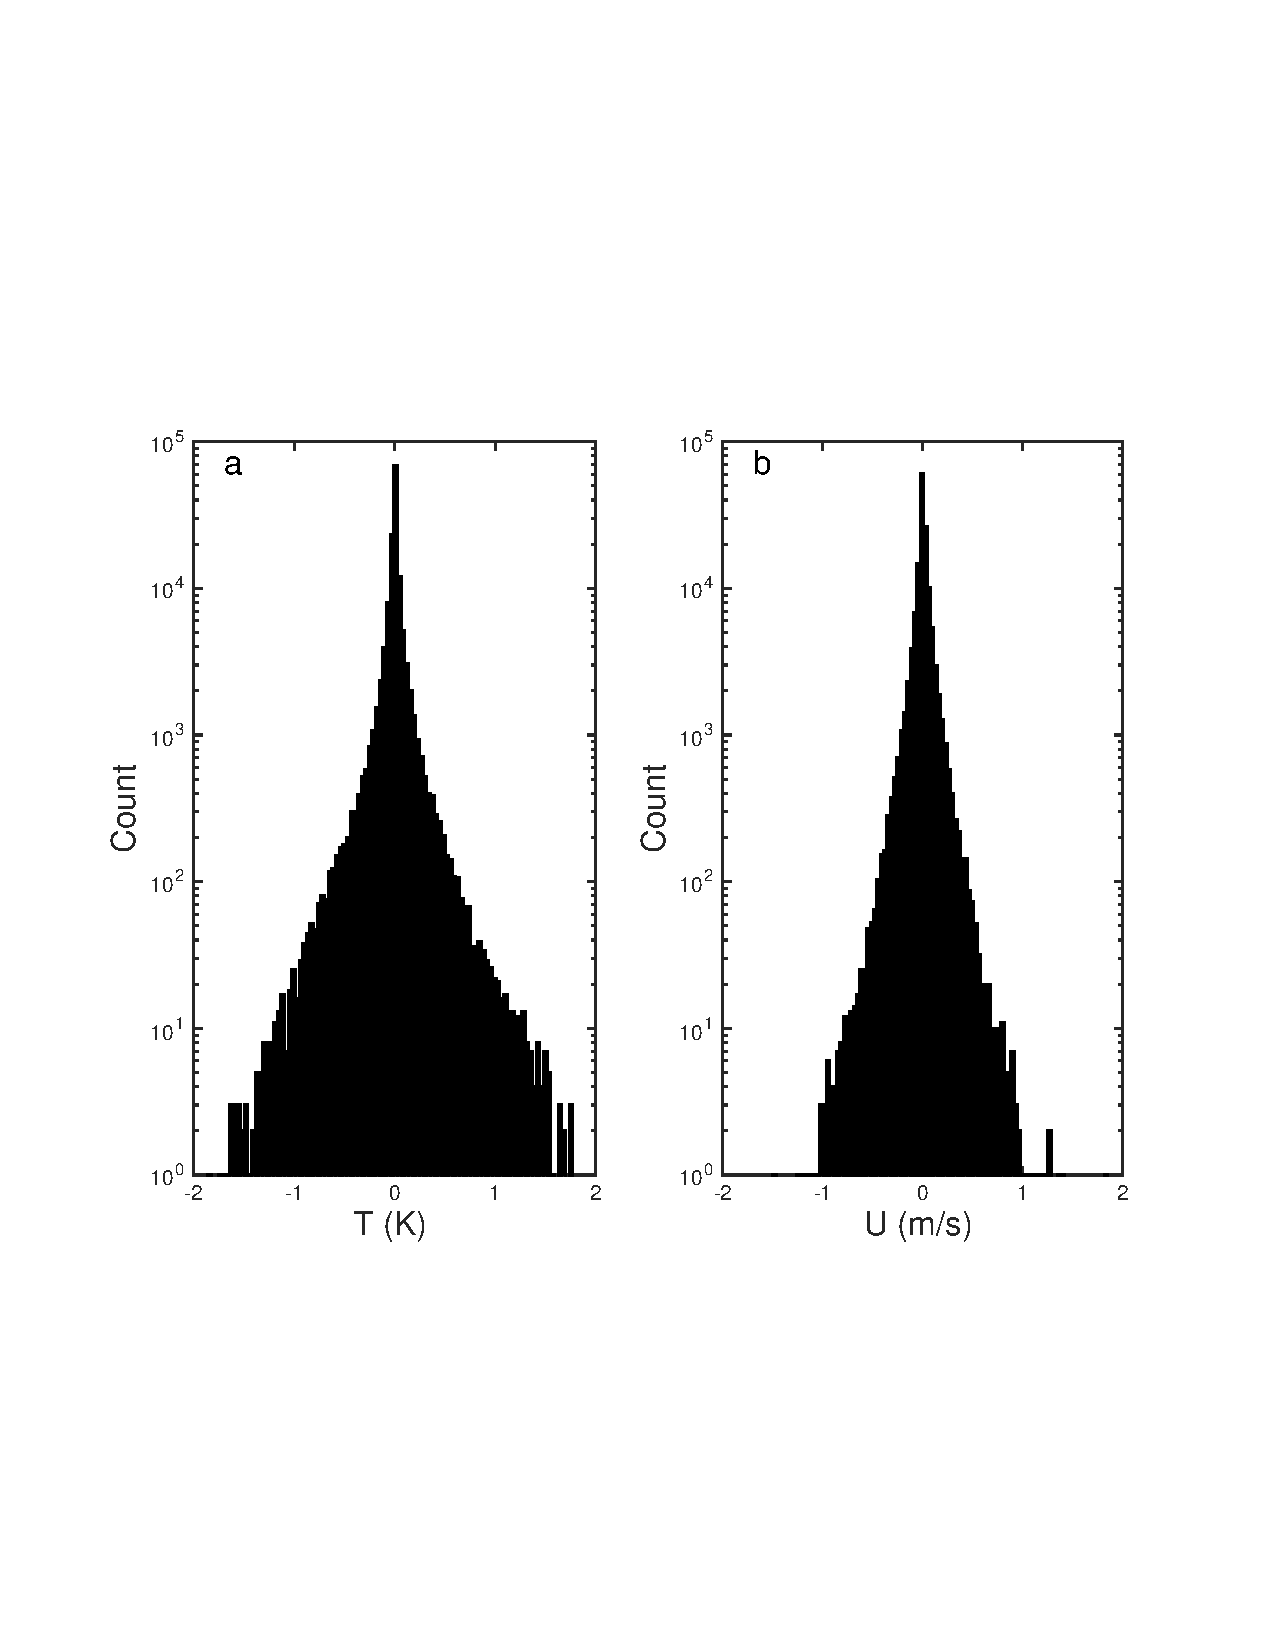
\includegraphics[clip,viewport=50 180 600 690,scale=.6]{figures/Fig03.pdf}
\caption{\label{Fig:Diffs} Differences between grid-point values of two Sandy simulations, (a) temperature and (b) zonal wind, valid 0000 UTC 28 Oct 2012 after 12 h. WRF executables differ only in a single compiler optimization flag. All grid points in the 3D volume are included. }
\end{center}
\end{figure}

A histogram of 3D grid-point differences between the two Sandy simulations, after 12 h of simulation time, shows that meaninful differences are present (Fig.\@ \ref{Fig:Diffs}). Although the majority of differences are small, the distribution tails indicate the onset of local perturbations. We know those perturbations will grow and propagate up-scale because the model equations are chaotic.  We can expect that higher-resolution grids, subject to more small-scale nonlinear processes, will lead to greater rates of growth of the differences between the two simulations.  Grids covering larger regions will be subject to greater rates of growth too, because the dynamical interactions cover a broader range of scales.

\section{Discussion}\label{sec:discussion}

This contribution presents a set of Docker containers intended to provide a basis for a WRF execution, and ancillary workflow components. As shown above, the container infrastructure offers many advantages for enabling research and education to be reproducible and more collaborative. A few more discussion points are summarized here.

The containers offer numerical and performance reproducibility in an easily, and rapidly, deployable framework that can enable collaborative research and education.  In section \ref{sec:uncertainty} we demonstrated the effects of compiler flags. Many NWP experiments reported in the literature focus on small differences between simulations, which are interpreted as physically relevant signals to be diagnosed. Although the majority of the differences may be physically relevant, the reproducibility provided by containers offers certainty. The extension is that uncertainty from sources besides numerical truncation can be isolated.  To further understand these issues, a study evaluating whether compiler optimizations, hardware variations, and parallel topologies lead to random-like or systematic errors would be helpful.

The containers enable the same kind of collaborative environment as a single community resource, but by making use of any resources locally available to individual researchers. In general, identical compilers and operating systems are not available to collaborating researchers, except when all participants are working on the same community computing resource and in the same environment. Numerical reproducibility even within collaborating groups is not straightforward. With containers, collaboration among groups of scientists that need to work on the same code, or produce parallel simulations with only small variations, is immediately enabled. Examples include ensemble forecasts run on distributed and inhomogeneous platforms by multiple people in different locations, model developers from different institutions who are working to improve a physics scheme, or researchers collaborating to better quantify an energy budget within the model. 

Educational activities clearly benefit from containers. Hands-on exercises are a valuable part of any student learning experience. Containers give instructors control over what parts of the modeling system students will experience directly. For example the WRF could be run initially as a ``black box,'' and then intermediate steps made accessible as students work through exercises. Software containers help standardize modules that can be easily shared amongst teaching colleagues with vastly different technology environments.

The broader science community has recently been placing a greater emphasis on reproducible research, and containers offer a key step toward reproducible NWP research. Published papers can cite a specific container version used in one part of a research flow (e.g.\@ the model, set of analysis tools, or a data container with initialization files). As long as that container revision exists and is accessible, research consumers can reproduce the results. This provides not only an unprecedented level of openness in NWP research, but also an easier way for researchers to build on published results. The resources below in section \ref{sec:resources} offer one component of the suite of tools needed to enable fully reproducible science. Metadata and analysis methods also need to be tracked and made available. Tools for that exist, and should be adopted by the NWP community as we go forward.



\section{Resources}\label{sec:resources}

This section provides links to on-line content, including documentation and open repositories for WRF-based containers. It will be complete in the final version, to ensure the links and content are stable.

%%%%%%%%%%%%%%%%%%%%%%%%%%%%%%%%%%%%%%%%%%%%%%%%%%%%%%%%%%%%%%%%%%%%%
% ACKNOWLEDGMENTS
%%%%%%%%%%%%%%%%%%%%%%%%%%%%%%%%%%%%%%%%%%%%%%%%%%%%%%%%%%%%%%%%%%%%%
%
\acknowledgments
Partial funding for this work is from the following: National Science Foundation awards ATM0753581/M0856145 to NCAR, and 1450488 to the University of California Santa Cruz. Sandia National Labs, and LANL/UCSC Institute for Scalable Scientific Data Management (ISSDM) also contributed funding. Cindy Halley-Gotway at NCAR produced the schematic in Fig.~\ref{Fig:Containers}. Amazon Web Services is acknowledged for providing an educational resource grant used for some of these investigations.

%%%%%%%%%%%%%%%%%%%%%%%%%%%%%%%%%%%%%%%%%%%%%%%%%%%%%%%%%%%%%%%%%%%%%
% APPENDIXES
%%%%%%%%%%%%%%%%%%%%%%%%%%%%%%%%%%%%%%%%%%%%%%%%%%%%%%%%%%%%%%%%%%%%%
%
% Use \appendix if there is only one appendix.
%\appendix

% Use \appendix[A], \appendix}[B], if you have multiple appendixes.
%\appendix[A]

%% Appendix title is necessary! For appendix title:
%\appendixtitle{}

%%% Appendix section numbering (note, skip \section and begin with \subsection)
% \subsection{First primary heading}

% \subsubsection{First secondary heading}

% \paragraph{First tertiary heading}

%% Important!
%\appendcaption{<appendix letter and number>}{<caption>} 
%must be used for figures and tables in appendixes, e.g.,
%
%\begin{figure}
%\noindent\includegraphics[width=19pc,angle=0]{figure01.pdf}\\
%\appendcaption{A1}{Caption here.}
%\end{figure}

%%%%%%%%%%%%%%%%%%%%%%%%%%%%%%%%%%%%%%%%%%%%%%%%%%%%%%%%%%%%%%%%%%%%%
% REFERENCES
%%%%%%%%%%%%%%%%%%%%%%%%%%%%%%%%%%%%%%%%%%%%%%%%%%%%%%%%%%%%%%%%%%%%%
% Make your BibTeX bibliography by using these commands:
 \bibliographystyle{ametsoc2014}
 \bibliography{refs.bib}


%%%%%%%%%%%%%%%%%%%%%%%%%%%%%%%%%%%%%%%%%%%%%%%%%%%%%%%%%%%%%%%%%%%%%
% TABLES
%%%%%%%%%%%%%%%%%%%%%%%%%%%%%%%%%%%%%%%%%%%%%%%%%%%%%%%%%%%%%%%%%%%%%
%% Enter tables at the end of the document, before figures.
%%
%

%%%%%%%%%%%%%%%%%%%%%%%%%%%%%%%%%%%%%%%%%%%%%%%%%%%%%%%%%%%%%%%%%%%%%
% FIGURES
%%%%%%%%%%%%%%%%%%%%%%%%%%%%%%%%%%%%%%%%%%%%%%%%%%%%%%%%%%%%%%%%%%%%%
%% Enter figures at the end of the document, after tables.
%%
%
%\begin{figure}[t]
%  \noindent\includegraphics[width=19pc,angle=0]{figure01.pdf}\\
%  \caption{Enter the caption for your figure here.  Repeat as
%  necessary for each of your figures. Figure from \protect\cite{Knutti2008}.}\label{f1}
%\end{figure}

%\clearpage
%\begin{figure}[t]
%  \noindent\includegraphics[width=19pc,angle=0]{../figs/WRFsolar.eps}\\
% \caption{\label{fig:wrfsolar}Sketch representing the physical processes that WRF-Solar is improving.}
%\end{figure}

\end{document}
